\documentclass[12pt]{article}

\usepackage{graphicx}

\begin{document}

\title{Homework 1: MapReduce}
\author{HeeHoon Kim}
\maketitle

\begin{figure}[ht]
    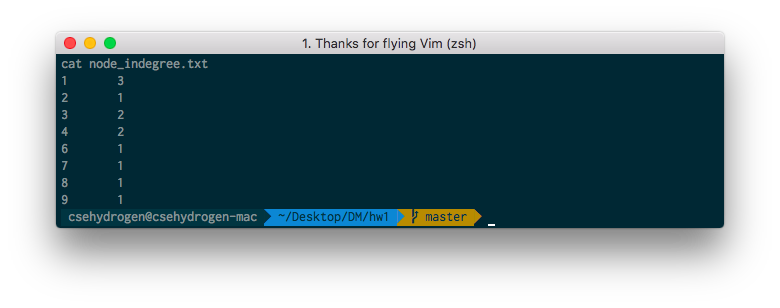
\includegraphics[width=\linewidth]{q1}
    \caption{After executing `make in'}
\end{figure}

\begin{figure}[ht]
    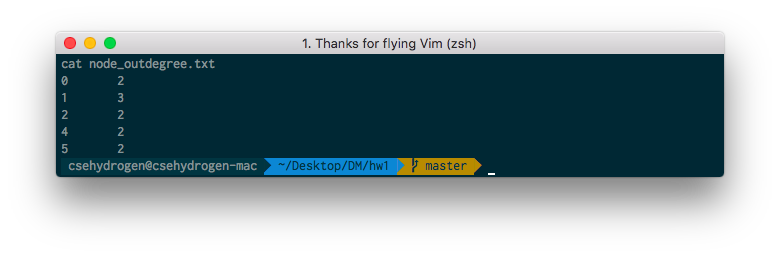
\includegraphics[width=\linewidth]{q2}
    \caption{After executing `make out'}
\end{figure}

\begin{figure}[ht]
    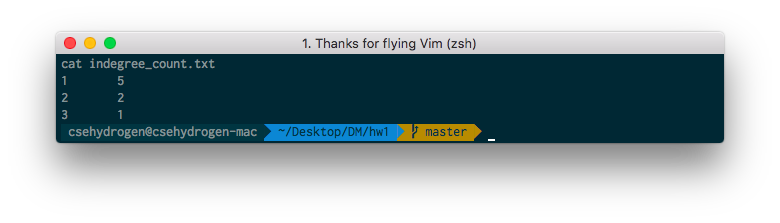
\includegraphics[width=\linewidth]{q3_1}
    \caption{After executing `make in\_dist'}
\end{figure}

\begin{figure}[ht]
    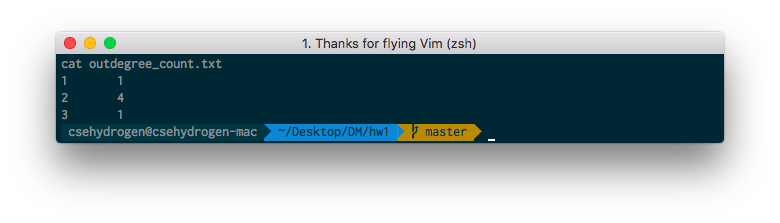
\includegraphics[width=\linewidth]{q3_2}
    \caption{After executing `make out\_dist'}
\end{figure}

\begin{figure}[ht]
    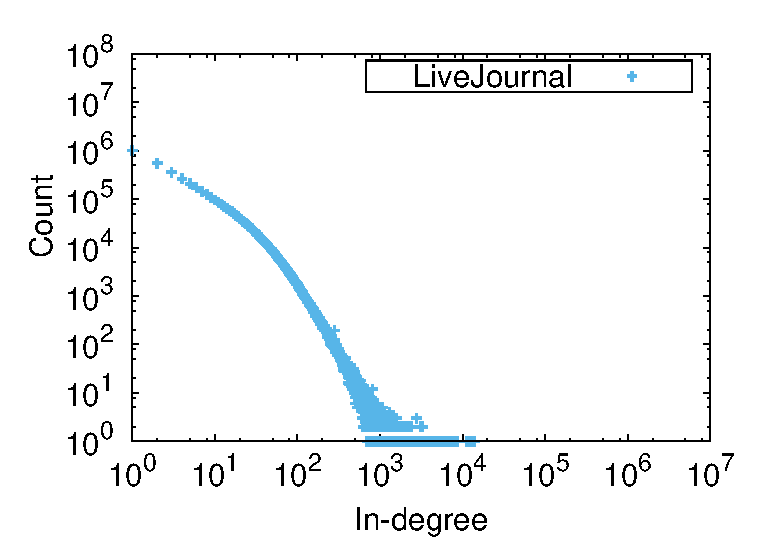
\includegraphics[width=0.5\linewidth]{q4_1}
    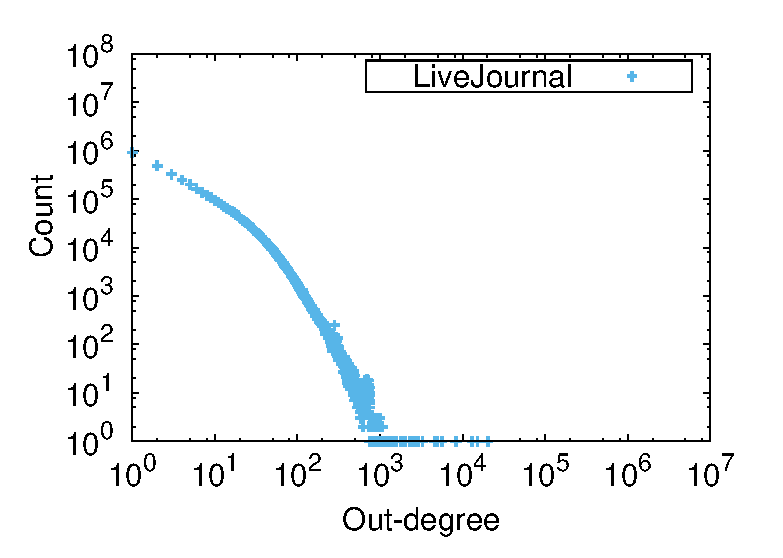
\includegraphics[width=0.5\linewidth]{q4_2}
    \caption{In-degree and Out-degree distributions of the LiveJournal dataset}
\end{figure}

\end{document}
